% Este trabalho está licenciado sob a Licença Creative Commons Atribuição-CompartilhaIgual 3.0 Não Adaptada. Para ver uma cópia desta licença, visite http://creativecommons.org/licenses/by-sa/3.0/ ou envie uma carta para Creative Commons, PO Box 1866, Mountain View, CA 94042, USA.

\documentclass[../livro.tex]{subfiles}  %%DM%%Escolher document class and options article, etc

\providecommand{\dir}{..}

%%%%%%%%%%%%%%%%%%%%%%%%%%%%%%%%%%%%%%%%%%%%%
%%%%%%%%%%%%INICIO DO DOCUMENTO%%%%%%%%%%%%%%
%%%%%%%%%%%%%%%%%%%%%%%%%%%%%%%%%%%%%%%%%%%%%

\begin{document}
	
\chapter{Semana 13}



\section{Método dos mínimos quadrados}

Sistemas lineares aparecem como modelos matemáticos de vários fenômenos e em várias situações. Acontece que alguns sistemas simplesmente não possuem soluções e ficamos sem saber como proceder. O \textbf{método dos mínimos quadrados} é uma técnica que nos permite, de forma aproximada, retirar alguma informação desses sistemas impossíveis. A terminologia se deve ao fato de que, como veremos, este método minimiza a soma dos quadrados dos erros obtidos na aproximação.

Como sabemos, resolver o sistema linear
\begin{equation}
A \vec{x} = \vec{b}
\end{equation} consiste em encontrar um vetor $\vec{x}$ que satisfaça a esta equação. Na terminologia que construimos ao longo do curso, é equivalente dizer que $\vec{b}$ pertence ao espaço coluna da matriz $A$, isto é, $\vec{b} \in \Col A$. Desta forma, não é possível resolver o sistema quando $\vec{b} \not\in \Col A$. Representamos esta situação na figura abaixo.
\begin{figure}[h!]
  \begin{center}
    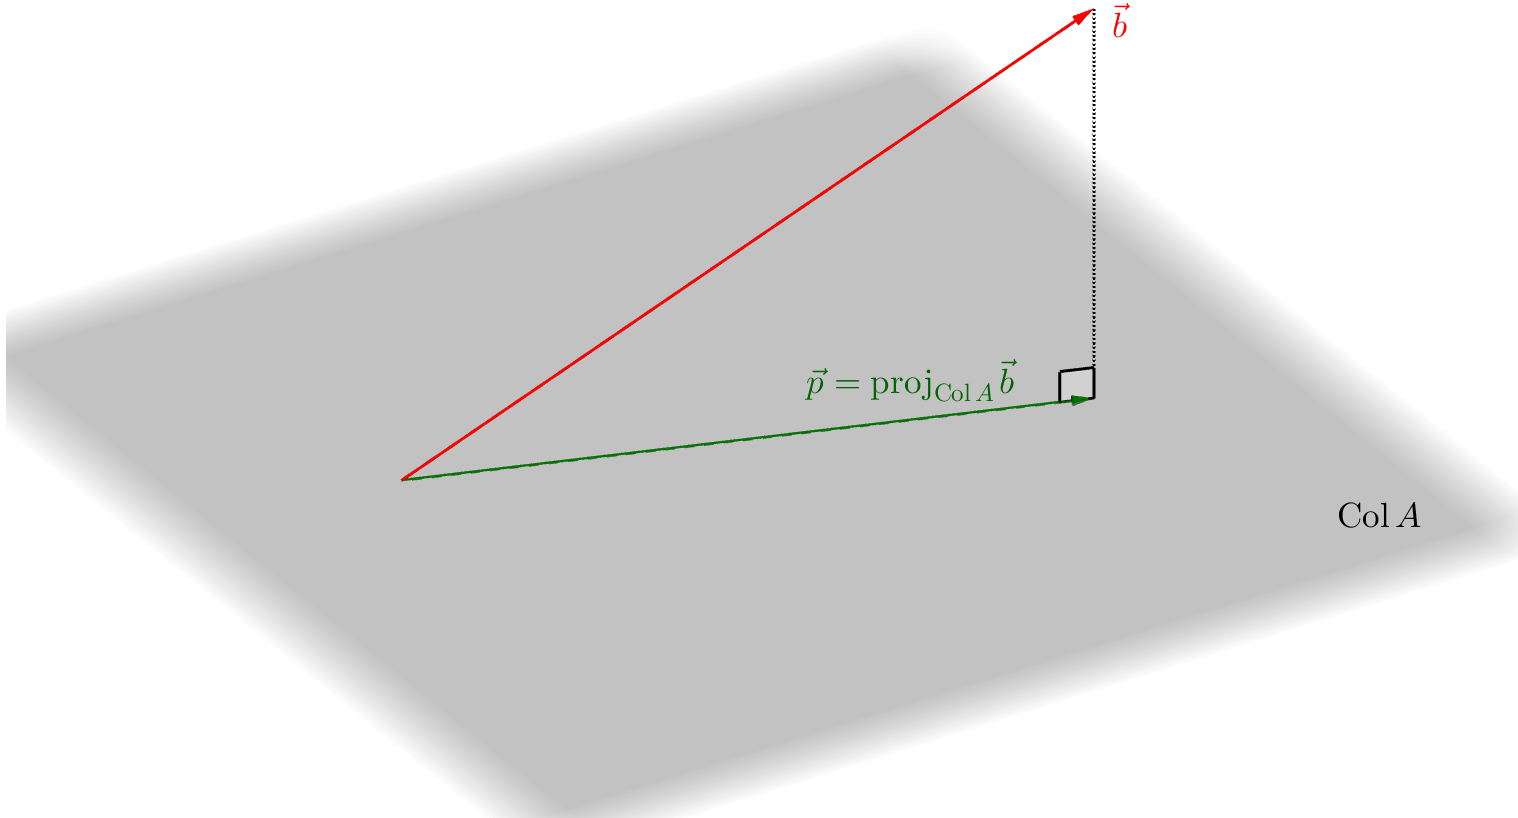
\includegraphics[width=0.8\linewidth]{\dir/Semana13/semana13-proj-col}
  \end{center}
\end{figure}

O método dos mínimos quadrados consiste em olhar para o vetor $\vec{p} = \proj_{\Col A} \vec{b}$ e resolver o sistema linear associado
\begin{equation}
A \vec{x} = \vec{p}.
\end{equation} Esta solução de $A \vec{x} = \vec{p}$ é chamada de \textbf{solução de mínimos quadrados}. A ideia é (ver figura) considerar o vetor pertencente a $\Col A$ que é o ``mais próximo'' possível de $\vec{b}$ e cujo sistema linear associado possua solução. Neste contexto, estamos pensando em mais próximo no sentido 
\begin{equation}
\| \vec{b} - \proj_{\Col A} \vec{b} \| \le \| \vec{b} - \vec{c} \|, \text{ para qualquer } \vec{c}\, \in \Col A,
\end{equation} isto é, no sentido de ser a projeção a melhor aproximação de $\vec{b}$ no espaço coluna de $A$. Escrevendo os vetores em coordenadas:
\begin{equation}
\vec{b} =
\begin{bmatrix}
  b_1 \\ b_2 \\ \vdots \\ b_n
\end{bmatrix} \quad \text{e} \quad 
\proj_{\Col A} \vec{b} =
\begin{bmatrix}
  p_1 \\ p_2 \\ \vdots \\ p_n
\end{bmatrix},
\end{equation} podemos definir o valor
\begin{equation}
\| \vec{b} - \proj_{\Col A} \vec{b} \| = \sqrt{\sum_{i=1}^n (b_i - p_i)^2}
\end{equation} como o \textbf{erro da aproximação} ou \textbf{erro  quadrático}. Logo, como anunciado, a soma dos quadrados dos erros obtidos cada componente é o mínimo possível.


\begin{example}\label{exp:minquad1}
  Considere o sistema linear
  \begin{equation}
  \left\{
    \begin{array}{ll}
      x_1 + x_2 - 2x_3 = 3 \\
      x_1  - 2x_3 = 2 \\
      x_2 + 2x_3 = 0 \\
      x_1 + x_2 - 2x_3 = 0
    \end{array}
  \right. \ \leftrightsquigarrow  \
  A \vec{x} = \begin{bmatrix}
    1 & 1 & -2 \\ 1 & 0 & -2 \\ 0 & 1 & 2 \\ -1 & -1 & 2
  \end{bmatrix}
  \begin{bmatrix}
    x_1 \\ x_2 \\ x_3
  \end{bmatrix} =
  \begin{bmatrix}
    3 \\ 2 \\ 0 \\ 0
  \end{bmatrix} = \vec{b}.
  \end{equation} Este sistema é claramente impossível, pois a primeira equação é inconsistente com a última. De forma mais automática, um passo no escalonamento da matriz aumentada associada revelaria a mesma conclusão:
  \begin{equation}
  [\, A \ | \ \vec{b} \, ] = \begin{bmatrix}
    1 & 1 & -2 & 3 \\ 1 & 0 & -2 & 2 \\ 0 & 1 & 2 & 0 \\ -1 & -1 & 2 & 0
  \end{bmatrix}   \sim
  \begin{bmatrix}
    1 & 1 & -2 & 3 \\ 1 & 0 & -2 & 2 \\ 0 & 1 & 2 & 0 \\ 0 & 0 & 0 & 3
  \end{bmatrix} .
  \end{equation} Vamos tentar encontrar, conforme descrito acima, uma solução de mínimos quadrados. Passos a serem realizados:
  \begin{itemize}
  \item Para calcular a projeção de $\vec{b}$ sobre $\Col A$, precisamos, em primeiro lugar, obter uma base ortogonal do espaço $\Col A$; isto pode ser feito pelo processo de Gram--Schmidt;
  \item Calcular a projeção $\vec{p} = \proj_{\Col A} \vec{b}$;
  \item Resolver o sistema linear $A \vec{x} = \vec{p}$.
  \end{itemize} Embora seja possível realizar estes três passos, temos de convir que seria muito trabalhoso. Por isto, vamos analisar um pouco mais da teoria para encontrar um método mais eficaz$. \ \lhd$
\end{example}

Suponhamos que:
\begin{itemize}
\item $A$ é uma matriz $m \times n$,
\item $\vec{x} \in \bR^n$,
\item $\vec{b} \in \bR^m$ e
\item o sistema $A \vec{x} = \vec{b}$ não possui solução.
\end{itemize} A solução de mínimos quadrados é a solução de $A \vec{x} = \vec{p}$, onde $\vec{p} = \proj_{\Col A} \vec{b}$. Observamos, por outro lado, que, sendo $\vec{p}\,$ a projeção sobre o espaço coluna de $A$, o vetor $\vec{b} - \vec{p}\,$ deve ser ortogonal a todos os elementos de $\Col A$. Em particular, se escrevermos $A$ em termos de suas colunas
\begin{equation}
A =
\begin{bmatrix}
  | & | &   & | \\
  \vec{a}_1 & \vec{a}_2 & \cdots  & \vec{a}_n \\
  | & | &   & |
\end{bmatrix}, \qquad \left( \text{que,  em particular, implica }
  A^T = \begin{bmatrix}
    \ \text{---} & \vec{a}_1  & \text{---} \ \\
    \ \text{---} & \vec{a}_2  & \text{---} \ \\
    \ & \vdots     &  \ \\
    \ \text{---} & \vec{a}_n  & \text{---}\ 
  \end{bmatrix}\right)
\end{equation} devemos ter
\begin{equation}
\vec{a}_j \cdot \big(\vec{b} - \vec{p}\big) = 0, \text{ para todo } j  \ \  \iff \ \
A^T (\vec{b} - \vec{p}) = \vec{0} \ \ \iff \ \ A^T \vec{b} = A^T \vec{p} = A^T A\vec{x}.
\end{equation} Esta última linha é válida porque o produto escalar $\vec{a}_j \cdot \big(\vec{b} - \vec{p}\big)$ é justamente a entrada $j$ do vetor obtido ao multiplicar $A^T(\vec{b} - \vec{p})$. Além disso, $A \vec{x} = \vec{p}.$

Concluimos, desta forma, que, se $\vec{x}$ é uma solução de mínimos quadrados, ou seja, se $A \vec{x} = \vec{p}$, então necessariamente
\begin{equation}\label{minquad}
  \boxed{A^T A\vec{x} = A^T \vec{b}.}
\end{equation}

\begin{exercise}[Teórico]
  Justifique que o conjunto de soluções do sistema \eqref{minquad} coincide com o conjunto das soluções de mínimos quadrados do sistema $A \vec{x} = \vec{b}$.
\end{exercise}

Tudo isto implica que podemos utilizar a equação \eqref{minquad} para encontrar as soluções de mínimos quadrados de $A \vec{x} = \vec{b}$. 

\begin{example}[De volta ao Exemplo \ref{exp:minquad1}]\label{exp:minquad2}
  Calculamos
  \begin{equation}
  A^T A =
  \begin{bmatrix}
    1 & 1 & 0 & -1 \\ 1 & 0 & 1 & -1 \\ -2 & -2 & 2 & 2
  \end{bmatrix}
  \begin{bmatrix}
    1 & 1 & -2 \\ 1 & 0 & -2 \\ 0 & 1 & 2 \\ -1 & -1 & 2
  \end{bmatrix} =
  \begin{bmatrix}
    3 & 2 & -6 \\ 2 & 3 & -2 \\ -6 & -2 & 16
  \end{bmatrix}
  \end{equation} e
  \begin{equation}
  A^T \vec{b} =
  \begin{bmatrix}
    1 & 1 & 0 & -1 \\ 1 & 0 & 1 & -1 \\ -2 & -2 & 2 & 2
  \end{bmatrix}
  \begin{bmatrix}
    3 \\ 2 \\ 0 \\ 0
  \end{bmatrix} =
  \begin{bmatrix}
    5 \\ 3 \\ -10
  \end{bmatrix}
  \end{equation} Para resolvermos o sistema $A^TA\vec{x} = A^T\vec{b}$, vamos escalonar a matriz aumentada associada:
  \begin{equation}
  \begin{bmatrix}
    3 & 2 & -6 & 5 \\
    2 & 3 & -2 & 3 \\
    -6 & -2 & 16 & -10
  \end{bmatrix} \sim
  \begin{bmatrix}
    3 & 2 & -6 & 5 \\
    0 & 5 &  6 & -1 \\
    0 & 2 &  4 & 0
  \end{bmatrix} \sim
  \begin{bmatrix}
    3 & 2 & -6 & 5 \\
    0 & 5 &  6 & -1 \\
    0 & 0 &  4 & 1
  \end{bmatrix}
  \end{equation} Logo,
  \begin{equation}
  \left\{
    \begin{array}{ll}
      3 x_1 + 2 x_2 - 6 x_3 = 5 \\
      5x_2 + 6 x_3 = -1 \\
      4x_3 = 1
    \end{array}
  \right..
  \end{equation} Assim,
  \begin{equation}
  x_3 = \frac{1}{4} \implies 5x_2 + 6 \cdot \frac{1}{4} = -1 \implies x_2 = -\frac{1}{2} \implies 3 x_1 - 1 - \frac{3}{2}  = 5 \implies x_1 = \frac{3}{2}.
  \end{equation} Portanto, uma solução de mínimos quadrados é
  \begin{equation}
  \begin{bmatrix}
    x_1 \\ x_2 \\ x_3
  \end{bmatrix} =
  \begin{bmatrix}
    3/2 \\ -1/2 \\ 1/4
  \end{bmatrix}.
  \end{equation} Observe como isto é muito menos trabalhoso do que o método que havíamos esquematizado no Exemplo \ref{exp:minquad1}$. \ \lhd$
\end{example}

\begin{exercise}
  Colocar em prática o método discutido no Exemplo \ref{exp:minquad1} e comparar o resultado com o que obtivemos no Exemplo \ref{exp:minquad2}.
\end{exercise}

\begin{remark}
  Caso a matriz $A$ já seja uma matriz ortogonal, podemos calcular projeções diretamente, pois uma base ortogonal para $\Col A$ já esté disponível desde o começo. Neste caso, ambos os métodos exigiriam um trabalho parecido.
\end{remark}

Nossa aproximação linear foi encontrada de modo a minimizar o erro quadrático. Para encontrar o erro, deveríamos calcular
\begin{equation}
\| \vec{b} - \proj_{\vec{\Col A}} \vec{b} \|.
\end{equation} No entanto, note que não precisamos calcular a projeção. Observando que a solução de mínimos quadrados satisfaz $A \vec{x} = \proj_{\vec{\Col A}} \vec{b}$, podemos calcular o erro por
\begin{equation}
\text{erro } = \| \vec{b} - A \vec{x} \|,
\end{equation} onde $\vec{x}$ é a solução de mínimos quadrados.

No Exemplo \ref{exp:minquad2} acima, podemos calcular o erro desta forma. De fato,
\begin{equation}
A \vec{x} = 
\begin{bmatrix}
  1 & 1 & -2 \\ 
  1 & 0 & -2 \\ 
  0 & 1 &  2 \\ 
  -1 & -1&  2
\end{bmatrix}
\begin{bmatrix}
  3/2 \\ -1/2 \\ 1/4
\end{bmatrix} = 
\begin{bmatrix}
  1/2 \\ 1 \\ 0 \\ -1/2
\end{bmatrix} \implies 
\vec{b} - A\vec{x} = 
\begin{bmatrix}
  5/2 \\ 1 \\ 0 \\ 1/2
\end{bmatrix}
\end{equation}
\begin{equation}
\implies \text{erro } = \| \vec{b} - A \vec{x} \| = \sqrt{\frac{25}{4} + 1 + \frac{1}{4}} = \frac{\sqrt{30}}{2} \simeq 2,74.
\end{equation}


% \newpage



\section{Regressão Linear Simples}

Vamos apresentar uma aplicação de algumas das técnicas do método de mínimos quadrados à Estatística ou Econometria. Uma \textbf{regressão linear simples} é uma equação, tipicamente da forma
\begin{equation}
y = a + b x,
\end{equation} para estimar os valores $(x,y)$ apenas conhecendo alguns valores específicos $(x_1, y_1), (x_2, y_2), \dots,$ $(x_k, y_k)$. A ideia é tentar capturar como que mudanças na variável independente $x$ afetam a variável dependente $y$ (neste caso, supondo que esta dependência é linear).

\begin{example}\footnote{Exemplo adaptado de \url{https://onlinecourses.science.psu.edu/stat501/node/257}}\label{exp:idade}
Com o intuito de analisar se é razoável supor que há um relação linear entre a idade de um motorista e quão longe ele consegue ver, uma empresa (Last Resource, Inc., Bellefonte, PA) coletou dados de 30 motoristas. Para simplificar as nossas contas, vamos listar abaixo \textit{apenas alguns} destes dados.
\begin{center}
 \begin{tabular}{|c|c|}
      \hline
      % after \\: \hline or \cline{col1-col2} \cline{col3-col4} ...
      Idade & Distância (em $m$) \\ \hline
      20 & 590 \\
      32 & 410 \\
      41 & 460 \\
      49 & 380 \\
      66 & 350 \\
      \hline
  \end{tabular}
\end{center} Podemos pensar em $y$ como a distância e em $x$ como a idade. Gostaríamos de achar uma relação linear da forma
\begin{equation}
  y = a + b x.
\end{equation} Desta forma, os dados obtidos implicam que  
\begin{equation}
\left\{
    \begin{array}{ll}
      b + 20 a = 590 \\
      b + 32 a = 410 \\
      b + 41 a = 460 \\
      b + 49 a = 380 \\
      b + 66 a = 350
    \end{array}
  \right. \ \ \leftrightsquigarrow \ \ \
  \begin{bmatrix}
    1 & 20 \\
    1 & 32 \\
    1 & 41 \\
    1 & 49 \\
    1 & 66 \\
  \end{bmatrix}
  \begin{bmatrix}
    a \\ b
  \end{bmatrix} =
  \begin{bmatrix}
    590 \\ 410 \\ 460 \\ 380 \\ 350
  \end{bmatrix}
  \end{equation} Ora, dificilmente um sistema linear com duas incógnitas e cinco equações terá solução (só terá solução se todos os pontos do conjunto de dados estiverem perfeitamente alinhados em uma reta!). Consequentemente, vamos procurar por uma solução de mínimos quadrados. Isto é \textbf{regressão linear simpes}.

  Denotando
  \begin{equation}
  A =
  \begin{bmatrix}
    1 & 20 \\
    1 & 32 \\
    1 & 41 \\
    1 & 49 \\
    1 & 66 \\
  \end{bmatrix} \quad \text{e} \quad
  \vec{b} =
  \begin{bmatrix}
    590 \\ 410 \\ 460 \\ 380 \\ 350
  \end{bmatrix}
  \end{equation} precisamos calcular
  \begin{equation}
  A^T A =
  \begin{bmatrix}
    1 & 1 & 1 & 1 & 1 \\
    20 & 32 & 41 & 49 & 66
  \end{bmatrix}
  \begin{bmatrix}
    1 & 20 \\
    1 & 32 \\
    1 & 41 \\
    1 & 49 \\
    1 & 66 \\
  \end{bmatrix} =
  \begin{bmatrix}
    5    & 208 \\
    208  & 9832  \\
  \end{bmatrix}
  \end{equation} e
  \begin{equation}
  A^T \vec{b} =
  \begin{bmatrix}
    1 & 1 & 1 & 1 & 1 \\
    20 & 32 & 41 & 49 & 66
  \end{bmatrix}
  \begin{bmatrix}
    590 \\ 410 \\ 460 \\ 380 \\ 350
  \end{bmatrix} =
  \begin{bmatrix}
    2190 \\ 85500
  \end{bmatrix}.
  \end{equation} Em seguida, a matriz associada aumentada pode ser reduzida por escalonamento:
  \begin{equation}
  [\, A^TA \ | \ \vec{b} \, ] =
  \begin{bmatrix}
    5    & 208 & 2190 \\
    208  & 9832 & 85500 \\
  \end{bmatrix} \sim
  \begin{bmatrix}
    1 & 0 & 468510/737 \\
    0 & 1 & -7005/1474 \\
  \end{bmatrix} \implies
  \left\{
    \begin{array}{ll}
      a \simeq 635.7 \\
      b \simeq -4.75
    \end{array}
  \right..
  \end{equation} Os números são feios, mas as contas feitas foram as que sempre fizemos ao escalonar uma matriz até sua forma escalonada reduzida.

  A conclusão é que a reta de mínimos quadrados que melhor aproxima os nossos dados é a reta
  \begin{equation}
  y = a + b x = 635.7 - 4.75 x.
  \end{equation} O erro de mínimos quadrados nesta aproximação (ou norma do resíduo) pode ser calculado como
  \begin{equation}
  A \vec{x} = \begin{bmatrix}
    1 & 20 \\
    1 & 32 \\
    1 & 41 \\
    1 & 49 \\
    1 & 66 \\
  \end{bmatrix}
  \begin{bmatrix}
    635.7 \\
    4.75 \\
  \end{bmatrix} \simeq
  \begin{bmatrix}
    730.7 \\
    787.7 \\
    830.45 \\
    868.45 \\
    949.2 \\
  \end{bmatrix} \simeq \proj_{\Col A} \vec{b} \implies \text{ erro } = \| \vec{b} - A\vec{x} \| \simeq 947.3
  \end{equation}
  \begin{figure}[h!]
    \begin{center}
      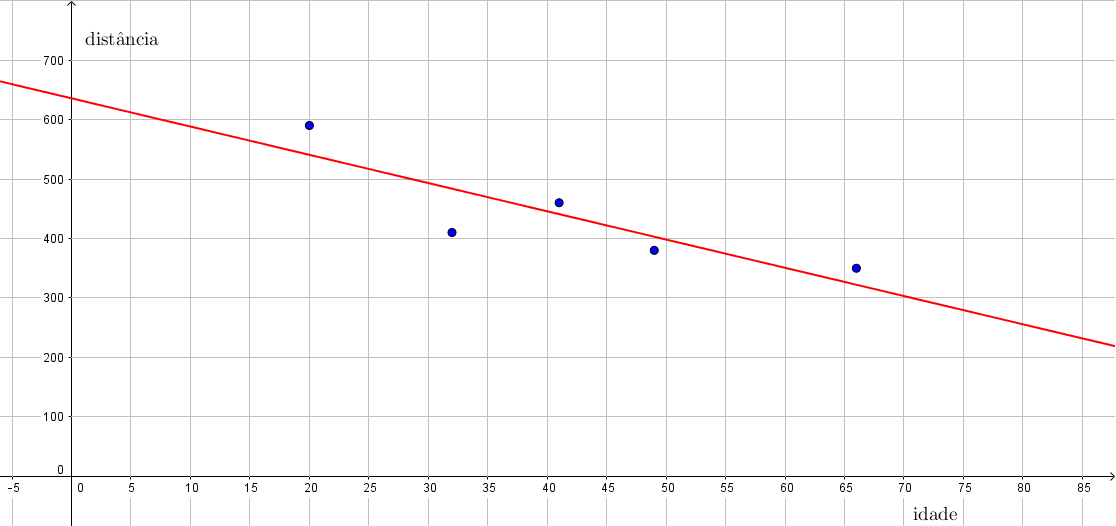
\includegraphics[width=1\linewidth]{\dir/Semana13/semana13-idade}
    \end{center}
  \end{figure}
 Na figura, mostramos um esboço da reta que melhor aproxima os dados deste exemplo$. \ \lhd$
\end{example}



De uma maneira geral, para encontrar uma \textbf{reta de melhor ajuste} a uma quantidade de pontos (dados coletados de algum problema)
\begin{equation}
(x_1, y_1), \ (x_2, y_2), \ \dots, (x_k, y_k),
\end{equation} devemos procurar pela solução $(a,b)$ de mínimos quadrados do sistema linear
\begin{equation}
\left\{
  \begin{array}{rl}
    a + b x_1 &\!\!\!\!\!= y_1  \\
    a + b x_2 &\!\!\!\!\!= y_2  \\
    \vdots &  \\
    a + b x_k &\!\!\!\!\!= y_k  \\
  \end{array}
\right. \quad \leftrightsquigarrow  \quad
\begin{bmatrix}
  1 & x_1 \\
  1 & x_2 \\
  \vdots & \vdots \\
  1 & x_k \\
\end{bmatrix}
\begin{bmatrix}
  a \\ b
\end{bmatrix} =
\begin{bmatrix}
  y_1 \\ y_2 \\ \vdots \\ y_k
\end{bmatrix}.
\end{equation} Vejamos um outro exemplo:

\begin{example}
  Encontrar a reta que melhor se ajusta aos pontos do plano
  \begin{equation}
  (1,2), \ \ (2,3), \ \ (2,4), \ \ (3,2), \ \ (4,3), \ \ (4,4), \ \ (5,3), \ \ (5,5), \ \ (6,4).
  \end{equation} Como vimos acima, podemos considerar
  \begin{equation}
  A =
  \begin{bmatrix}
    1 & 1 \\
    1 & 2 \\
    1 & 2 \\
    1 & 3 \\
    1 & 4 \\
    1 & 4 \\
    1 & 5 \\
    1 & 5 \\
    1 & 6 \\
  \end{bmatrix} \ \ \text{e} \ \
  \vec{b} =
  \begin{bmatrix}
    2\\3\\4\\2\\3\\4\\3\\5\\4
  \end{bmatrix}
  \end{equation} Assim,
  \begin{equation}
  A^T A =
  \begin{bmatrix}
    9  & 32  \\
    32  & 136
  \end{bmatrix}  \ \ \text{e} \ \
  A^T \vec{b} =
  \begin{bmatrix}
    30\\114
  \end{bmatrix}.
  \end{equation} A solução de mínimos quadrados, que é a solução de $A^T A \vec{x} = A^T\vec{b}$, é dada por
  \begin{equation}
  b = 54/25 = 2.16, \\ a = 33/100 = 0.33.
  \end{equation} A reta procurada é portanto $y = 0.33 x + 2.16$.
  \begin{figure}[h!]
    \begin{center}
      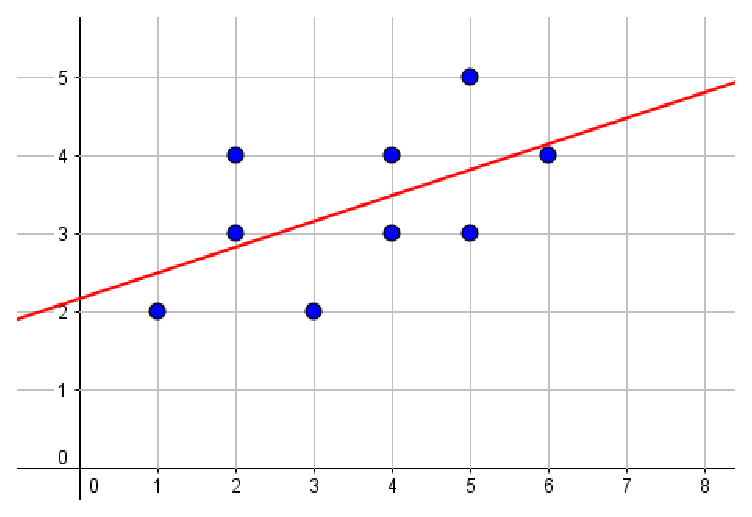
\includegraphics[width=0.5\linewidth]{\dir/Semana13/semana13-reta}
    \end{center}
  \end{figure}
\end{example}


\section{Regressão não linear}


Podemos também procurar (em contraste com a subseção anterior) por funções não lineares que se ajustem a um conjunto de pontos. Por exemplo, dado um certo conjunto de pontos
\begin{equation}
(x_1, y_1), \ (x_2, y_2), \ \dots, (x_k, y_k),
\end{equation} vamos procurar por uma parábola
\begin{equation}
y = a + bx + cx^2
\end{equation} que melhor se ajuste a este conjunto de pontos, no sentido de que a soma dos quadrados dos erros seja a menor possível. Isto corrensponde a procurar pela solução $(a,b, c)$ de mínimos quadrados do seguinte sistema linear
\begin{equation}
\left\{
  \begin{array}{rl}
    a + b x_1 + c x_1^2 &\!\!\!\!\!= y_1  \\
    a + b x_2 + c x_2^2 &\!\!\!\!\!= y_2  \\
    \vdots &  \\
    a + b x_k + c x_k^2 &\!\!\!\!\!= y_k  \\
  \end{array}
\right. \quad \leftrightsquigarrow  \quad
\begin{bmatrix}
  1 & x_1 & x_1^2 \\
  1 & x_2 & x_2^2 \\
  \vdots & \vdots \\
  1 & x_k & x_k^2 \\
\end{bmatrix}
\begin{bmatrix}
  a \\ b \\ c
\end{bmatrix} =
\begin{bmatrix}
  y_1 \\ y_2 \\ \vdots \\ y_k
\end{bmatrix}.
\end{equation} Vejamos como ficaria a parábola que se ajusta aos dados do Exemplo \ref{exp:idade}:

\begin{example}
  Nossos pontos no Exemplo \ref{exp:idade} são
  \begin{equation}
  (20, 590), \ (32, 410), \ (41, 460), \ (49, 380), \ (66, 350).
  \end{equation} Para encontrar a parábola de melhor ajuste como acima, devemos procurar pela solução de mínimos quadrados do sistema
  \begin{equation}
  \begin{bmatrix}
    1 & 20 & 400 \\
    1 & 32 & 1024 \\
    1 & 41 & 1681 \\
    1 & 49 & 2401 \\
    1 & 66 & 4356 \\
  \end{bmatrix}
  \begin{bmatrix}
    a \\ b \\ c
  \end{bmatrix} =
  \begin{bmatrix}
    590 \\ 410 \\ 460 \\ 380 \\ 350
  \end{bmatrix} \ \leftrightsquigarrow \ A \vec{x} = \vec{b}.
  \end{equation} Calculamos (com o auxílio de uma calculadora)
  \begin{equation}
  A^T A =
  \begin{bmatrix}
    1 & 1 & 1 & 1 & 1 \\
    20 & 32 & 41 & 49 & 66 \\
    400 & 1024 & 1681 & 2401 & 4356 \\
  \end{bmatrix}
  \begin{bmatrix}
    1 & 20 & 400 \\
    1 & 32 & 1024 \\
    1 & 41 & 1681 \\
    1 & 49 & 2401 \\
    1 & 66 & 4356 \\
  \end{bmatrix} =
  \begin{bmatrix}
    5 & 208 & 9862 \\
    208 & 9862 & 514834 \\
    9862 & 514834 & 28773874 \\
  \end{bmatrix},
  \end{equation}
  \begin{equation}
  A^T A =
  \begin{bmatrix}
    1 & 1 & 1 & 1 & 1 \\
    20 & 32 & 41 & 49 & 66 \\
    400 & 1024 & 1681 & 2401 & 4356 \\
  \end{bmatrix}
  \begin{bmatrix}
    590 \\ 410 \\ 460 \\ 380 \\ 350
  \end{bmatrix} =
  \begin{bmatrix}
    2190 \\ 85500 \\ 3866080
  \end{bmatrix}
  \end{equation} e resolvemos (escalonando, por exemplo, com o auxílio de um computador)
  \begin{equation}
  \begin{bmatrix}
    5 & 208 & 9862 & 2190 \\
    208 & 9862 & 514834 & 85500 \\
    9862 & 514834 & 28773874 & 3866080 \\
  \end{bmatrix} \sim
  \begin{bmatrix}
    1 & 0 & 0 & 28482529840/35036713 \\
    0 & 1 & 0 & -1505841055/105110139 \\
    0 & 0 & 1 & 11779375/105110139 \\
  \end{bmatrix}.
  \end{equation} 
  Logo, aproximando estas frações, obtemos
  \begin{equation}
  \left\{
    \begin{array}{ll}
      a \simeq 812.934 \\
      b \simeq -14.326 \\
      c \simeq  0.112 \\
    \end{array}
  \right.
  \end{equation} 
  \begin{figure}[h!]
  	\begin{center}
  		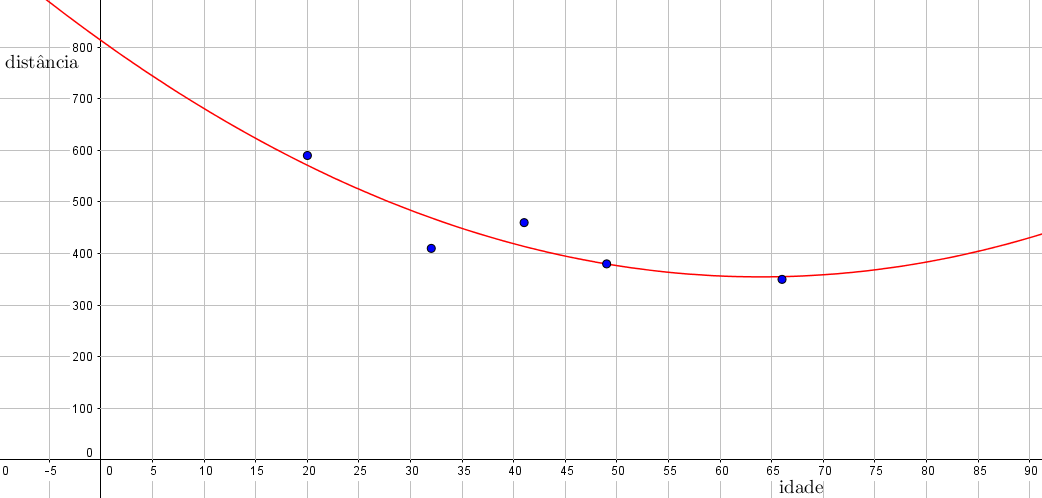
\includegraphics[width=1\linewidth]{\dir/Semana13/semana13-idade-parabola}
  	\end{center}
  \end{figure}
  e a parábola desejada é, aproximadamente
  \begin{equation}
  y = 812.934 - 14.326 x + 0.112 x^2.
  \end{equation}
  

  \noindent Observamos que, apesar de o erro quadrático ser provavelmente menor neste exemplo, esta parábola se torna crescente a partir de um certo momento, fazendo com que o modelo não seja tão razoável para idades maiores. Por exemplo, é pouco provável que (na média), pessoas com 95 anos vejam a uma distância maior do que pessoas de 65 anos, como sugere a parábola acima.
\end{example}



\section{Regressão linear múltipla}

Uma \textbf{regressão linear múltipla} é o problema análogo à regressão linear simples no caso em que a variável dependente pode depender de mais fatores independentes. Tipicamente, queremos encontrar uma equação afim que melhor se ajusta a alguns dados conhecidos.

No caso especial em que $y$ depende de apenas outros dois fatores, escreveremos
\begin{equation}
z = a + b x + c y,
\end{equation} que, geometricamente, representa um plano no espaço tridimensional $\bR^3$. Seja agora uma conjunto de dados:
\begin{equation}
(x_1, y_1, z_1), \ (x_1, y_1, z_1), \dots, (x_k, y_k, z_k).
\end{equation} Queremos encontrar coeficientes $(a,b,c)$ que satisfaçam:
\begin{equation}
\left\{
  \begin{array}{c}
    a + b x_1 + c y_1 = z_1 \\
    a + b x_2 + c y_2 = z_2 \\
    \vdots \\
    a + b x_k + c y_k = z_k \\
  \end{array}
\right. \quad \leftrightsquigarrow \quad
\begin{bmatrix}
  1 & x_1 & y_1 \\
  1 & x_2 & y_2 \\
  \vdots & \vdots & \vdots \\
  1 & x_k & y_k \\
\end{bmatrix}
\begin{bmatrix}
  a \\ b \\ c
\end{bmatrix} =
\begin{bmatrix}
  z_1 \\ z_2 \\ \vdots \\ z_k
\end{bmatrix}.
\end{equation} Quanto maior o número de dados, mais provável de o sistema ser impossível (podemos fazer a analogia geométrica de que por três pontos não colineares no espaço passa um único plano; se aumentarmos o número de pontos, mais difícil que haja um plano contendo todos eles). Por isto, procuramos por uma solução de mínimos quadrados.



\begin{example}
  Uma pesquisa com $214$ mulheres em uma universidade americana\footnote{Referência: \verb"\url{https://onlinecourses.science.psu.edu/stat501/node/292}"} coletou informações sobre a altura das participantes, assim como a altura de seus pais. Abaixo, listamos \textit{apenas alguns destes dados}, para que nossas contas não fiquem tão extensas. Fizemos também uma mudança de unidades nas alturas (de polegadas) para centímetros,
  \begin{center}
    \begin{tabular}{|c|c|c|}
      \hline
      % after \\: \hline or \cline{col1-col2} \cline{col3-col4} ...
      Altura & Altura Mãe & Altura Pai \\ \hline
      152 & 155 & 165 \\
      162 & 155 & 160 \\
      165 & 170 & 173 \\
      170 & 163 & 183 \\
      173 & 168 & 183 \\
      183 & 165 & 183 \\
      \hline
    \end{tabular}
  \end{center} Queremos encontrar uma solução de mínimos quadrados para o sistema linear
  \begin{equation}
  \begin{bmatrix}
    1 & 155 & 165 \\
    1 & 155 & 160 \\
    1 & 170 & 173 \\
    1 & 163 & 183 \\
    1 & 168 & 183 \\
    1 & 165 & 183 \\
  \end{bmatrix}
  \begin{bmatrix}
    a \\ b \\ c
  \end{bmatrix} =
  \begin{bmatrix}
    152  \\
    162  \\
    165  \\
    170  \\
    173  \\
    183  \\
  \end{bmatrix} \ \leftrightsquigarrow \ A \vec{x} = \vec{b}.
  \end{equation} Calculamos
  \begin{equation}
  A^TA =
  \begin{bmatrix}
    1 & 1 & 1 & 1 & 1 & 1 \\
    155 & 155 & 170 & 163 & 168 & 165 \\
    165 & 160 & 173 & 183 & 183 & 183 \\
  \end{bmatrix}
  \begin{bmatrix}
    1 & 155 & 165 \\
    1 & 155 & 160 \\
    1 & 170 & 173 \\
    1 & 163 & 183 \\
    1 & 168 & 183 \\
    1 & 165 & 183 \\
  \end{bmatrix} =
  \begin{bmatrix}
    6 & 976 & 1047 \\
    976 & 158968 & 170553 \\
    1047 & 170553 & 183221 \\
  \end{bmatrix}
  \end{equation} e
  \begin{equation}
  A^T \vec{b} =
  \begin{bmatrix}
    1 & 1 & 1 & 1 & 1 & 1 \\
    155 & 155 & 170 & 163 & 168 & 165 \\
    165 & 160 & 173 & 183 & 183 & 183 \\
  \end{bmatrix}
  \begin{bmatrix}
    152  \\
    162  \\
    165  \\
    170  \\
    173  \\
    183  \\
  \end{bmatrix} =
  \begin{bmatrix}
    1005  \\
    163689  \\
    175803 \\
  \end{bmatrix}.
  \end{equation} Por escalonamento,
  \begin{equation}
  \begin{bmatrix}
    6    & 976    & 1047   & 1005     \\
    976  & 158968 & 170553 & 163689   \\
    1047 & 170553 & 183221 & 175803   \\
  \end{bmatrix} \sim
  \begin{bmatrix}
    1 & 0 & 0  & 2154573/145769 \\
    0 & 1 & 0  & 14475/145769   \\
    0 & 0 & 1  & 114081/145769  \\
  \end{bmatrix} \implies
  \left\{
    \begin{array}{ll}
      a \simeq 14.781  \\
      b \simeq  0.099  \\
      c \simeq  0.783  \\
    \end{array}
  \right.
  \end{equation} A equação de melhor ajuste procurada é, portanto, aproximadamente,
  \begin{equation}
  z \simeq 14.781 + 0.099 x + 0.783 y.
  \end{equation} Tente calcular sua altura $z$ a partir da altura de sua mãe $x$ e de seu pai $y$. O teste deve funcionar melhor para mulheres! Além disso, a aproximação linear deve ser melhor utilizando mais dados nos cálculos.
  \begin{figure}[h!]
    \begin{center}
      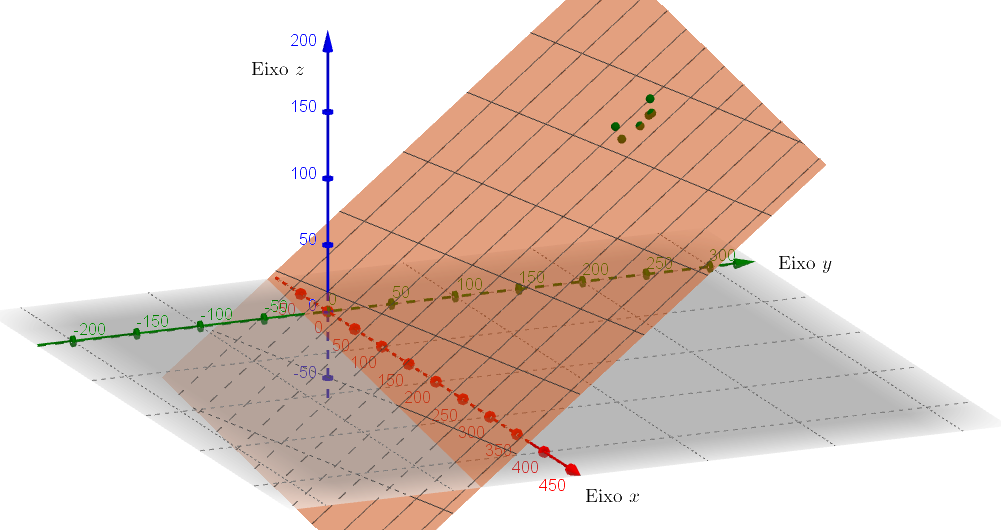
\includegraphics[width=1\linewidth]{\dir/Semana13/semana13-alturas}
    \end{center}
  \end{figure}
\end{example}

\section{Fatoração QR e Mínimos Quadrados}

Vimos que o processo de Gram-Schmidt nos permite escrever uma matriz $A$ cujas linhas são linearmente independentes na forma $A=QR$, onde $Q$ é uma matriz ortogonal, $R$ é triangular superior invertível, e as colunas de $Q$ formam uma base ortonormal para o espaço-coluna de $A$. Chamamos esta fatoração de $A$ de fatoração QR. 

A fatoração QR tem uma importante aplicação na solução de problemas em mínimos quadrados. Ocorre que, em muitos problemas, a matriz $A^T A$ é uma matriz {\it mal-condicionada}, ou seja, uma matriz que é muito sensível aos erros de aproximação cometidos em cálculos numéricos usualmente executados no tratamento de problemas aplicados. 
Os exemplos que virão a seguir nos mostram situações em que há uma grande variação de magnitude entre as entradas da matriz $A^T A$, e isto costuma ser fonte de instabilidade numérica.

Para isso, a fatoração QR oferece uma solução alternativa em mínimos quadrados para um sistema linear $A\vec{x}= \vec{b}$:
se $A=QR$, então 
\begin{equation}
A^T=R^T Q^T
\ \ \mbox{ que implica em } \ \
A^T A= R^T Q^T Q R= R^T R,
\end{equation}
onde usamos o fato de que $Q^{-1}=Q^T$.
Assim as equações normais $A^T A \vec{x} = A^T \vec{b}$ se reduzem a 
\begin{equation} R^T R \vec{x} = R^T Q^T \vec{b}.\end{equation}
Ainda, como $R$ é invertível podemos eliminar (cancelar) $R^T$ na equação acima, %ficando com a seguinte expressão para a solução em mínimos quadrados
obtendo o seguinte:
\begin{theorem}
	Se $A=QR$ com $Q$ ortogonal e $R$ triangular superior invertível, então 
	a solução em mínimos quadrados do sistema $A\vec{x}= \vec{b}$ é única e dada pela solução do sistema
	\begin{equation}  R \vec{x} =  Q^T \vec{b}.\end{equation}
\end{theorem}

Note que o fato de $R$ ser triangular superior torna a resolução do sistema acima pouco custosa do ponto de vista computacional. Alternativamente, temos uma expressão explícita para solução em mínimos quadrados: \begin{equation}   \vec{x} = R^{-1} Q^T \vec{b}.\end{equation}

É importante notar que existem algoritmos para fatoração QR que são \textit{numéricamente estáveis}, ou seja pouco suscetiveis a erros de aproximação ou arredondamento. Tais algorimos são diferentes do processo de Gram Schmidt usual.





\end{document} 